\documentclass[aspectratio=169]{beamer}
\usepackage{amsmath}
\usepackage{amssymb}
\usepackage{graphicx}
\usepackage{tcolorbox}
\usepackage{booktabs}
\usepackage{colortbl}
\usepackage{xcolor}
\usepackage{tikz}
\usetikzlibrary{arrows.meta,calc,decorations.pathreplacing}
\usepackage[utf8]{inputenc}

% Custom colors
\definecolor{primary}{RGB}{41, 128, 185}
\definecolor{secondary}{RGB}{52, 152, 219}
\definecolor{accent}{RGB}{231, 76, 60}
\definecolor{lightgray}{RGB}{236, 240, 241}

% Theme customization
\usetheme{Madrid}
\usecolortheme{whale}
\setbeamercolor{structure}{fg=primary}
\setbeamercolor{background canvas}{bg=white}
\setbeamercolor{normal text}{fg=black}

\title{Chapter 4.3: Solving Radical Functions}
\subtitle{Pre-Calculus 11 - Lesson 3}
\author{Created by Yi-Chen Lin}
\date{\today}

\begin{document}

\begin{frame}
\titlepage
\end{frame}

% Overview
\begin{frame}{Overview: Solving Radical Functions}
\begin{tcolorbox}[colback=lightgray,colframe=primary,title=Key Concepts]
\footnotesize
\begin{itemize}
  \item A root (radical) function is like a sideways parabola (e.g., $y=\sqrt{x}$)
  \item The domain starts where the radicand is zero
  \item To solve radical equations: isolate, square both sides, solve, and check for extraneous roots
\end{itemize}
\end{tcolorbox}
\end{frame}

% I) Understanding Root Functions
\begin{frame}{I) Understanding Root Functions}
\begin{tcolorbox}[colback=lightgray,colframe=primary,title=Key Points]
\footnotesize
\begin{itemize}
  \item $y=\sqrt{x}$ is the top half of a sideways parabola
  \item $x=y^2$ is a horizontal parabola
  \item The graph of $y=\sqrt{x}$ starts at $x=0$ and only exists for $x\geq0$
\end{itemize}
\end{tcolorbox}
\vspace{0.5em}
\begin{center}
\begin{tikzpicture}[scale=0.8]
  \draw[->] (-1,0) -- (5,0) node[right] {$x$};
  \draw[->] (0,-1) -- (0,3) node[above] {$y$};
  \draw[thick,primary,domain=0:4,samples=100] plot (\x,{sqrt(\x)});
  \node[below left] at (0,0) {0};
  \node[above] at (2,1.4) {$y=\sqrt{x}$};
\end{tikzpicture}
\end{center}
\end{frame}

% II) Where does the radical function begin?
\begin{frame}{II) Where Does the Radical Function Begin?}
\begin{tcolorbox}[colback=lightgray,colframe=primary,title=Domain of Radical Functions]
\footnotesize
\begin{itemize}
  \item The function $y=\sqrt{x-a}$ begins at $x=a$
  \item The function $y=\sqrt{2x+4}$ begins at $x=-2$
  \item The function $y=\sqrt{6-x}$ begins at $x=6$
\end{itemize}
\end{tcolorbox}
\vspace{0.5em}
\begin{columns}
\column{0.5\textwidth}
\begin{tikzpicture}[scale=0.7]
  \draw[->] (-3,0) -- (5,0) node[right] {$x$};
  \draw[->] (0,-1) -- (0,3) node[above] {$y$};
  \draw[thick,primary,domain=-2:4,samples=100] plot (\x,{sqrt(\x+2)});
  \node[below left] at (0,0) {0};
  \node[above] at (2,1.7) {$y=\sqrt{x+2}$};
\end{tikzpicture}
\column{0.5\textwidth}
\begin{tikzpicture}[scale=0.7]
  \draw[->] (-1,0) -- (7,0) node[right] {$x$};
  \draw[->] (0,-1) -- (0,3) node[above] {$y$};
  \draw[thick,primary,domain=0:6,samples=100] plot (\x,{sqrt(6-\x)});
  \node[below left] at (0,0) {0};
  \node[above] at (2,1.7) {$y=\sqrt{6-x}$};
\end{tikzpicture}
\end{columns}
\end{frame}

% III) Steps for Solving Radical Equations
\begin{frame}{III) Steps for Solving Radical Equations}
\begin{tcolorbox}[colback=lightgray,colframe=primary,title=Solving Steps]
\footnotesize
\begin{enumerate}
  \item Isolate the radical
  \item Square both sides to eliminate the radical
  \item Solve for $x$
  \item Check for extraneous roots by plugging back into the original equation
\end{enumerate}
\end{tcolorbox}
\end{frame}

% Example: Solving a Radical Equation
\begin{frame}{Example: Solving a Radical Equation}
\begin{tcolorbox}[colback=lightgray,colframe=accent,title=Example]
\footnotesize
Solve $\sqrt{2x-1} = 4$.
\begin{align*}
  &\sqrt{2x-1} = 4 \\
  &2x-1 = 16 \\
  &2x = 17 \\
  &x = 8.5
\end{align*}
Check: $\sqrt{2\times8.5-1} = \sqrt{17-1} = \sqrt{16} = 4$ (valid)
\end{tcolorbox}
\vspace{0.5em}
\begin{center}
\begin{tikzpicture}[scale=0.7]
  \draw[->] (-1,0) -- (10,0) node[right] {$x$};
  \draw[->] (0,-1) -- (0,5) node[above] {$y$};
  \draw[thick,primary,domain=0:9,samples=100] plot (\x,{sqrt(2*\x-1)});
  \draw[thick,accent] (8.5,4) circle (0.15);
  \node[below] at (8.5,0) {$8.5$};
  \node[left] at (0,4) {$4$};
  \node[above] at (6,3) {$y=\sqrt{2x-1}$};
\end{tikzpicture}
\end{center}
\end{frame}

% Practice: Solve radical equations
\begin{frame}{Practice: Solve the Radical Equations}
\begin{tcolorbox}[colback=lightgray,colframe=accent,title=Practice Problems]
\footnotesize
\begin{enumerate}
  \item $\sqrt{x+4} = 6$
\end{enumerate}
\begin{enumerate}
  \item $\sqrt{2x-3} = 5$
\end{enumerate}
\begin{enumerate}
  \item $\sqrt{3x+1} = x-2$
\end{enumerate}
\begin{enumerate}
  \item $\sqrt{x-1} + 2 = 7$
\end{enumerate}
\end{tcolorbox}
\end{frame}

% 1a
\begin{frame}{Practice: Solve the Radical Equations - Solution 1a}
\begin{tcolorbox}[colback=lightgray,colframe=primary,title=Solution 1a]
\footnotesize
\begin{columns}[T]
\column{0.55\textwidth}
\textbf{Solving:}

\begin{align*}
  &\sqrt{x+4} = 6 \\
  &(\sqrt{x+4})^2 = 6^2 \\
  &x+4 = 36 \\
  &x = 32
\end{align*}

\column{0.45\textwidth}
\textbf{Checking:}

\begin{align*}
  &\sqrt{32+4} = \sqrt{36} = 6 \\
  &\text{True!}
\end{align*}
\end{columns}
\end{tcolorbox}
\end{frame}

% 1b
\begin{frame}{Practice: Solve the Radical Equations - Solution 1b}
\begin{tcolorbox}[colback=lightgray,colframe=primary,title=Solution 1b]
\footnotesize
\begin{columns}[T]
\column{0.55\textwidth}
\textbf{Solving:}

\begin{align*}
  &\sqrt{2x-3} = 5 \\
  &(\sqrt{2x-3})^2 = 5^2 \\
  &2x-3 = 25 \\
  &2x = 28 \\
  &x = 14
\end{align*}

\column{0.45\textwidth}
\textbf{Checking:}

\begin{align*}
  &\sqrt{2(14)-3} = \sqrt{28-3} = \sqrt{25} = 5 \\
  &\text{True!}
\end{align*}
\end{columns}
\end{tcolorbox}
\end{frame}

% 1c
\begin{frame}{Practice: Solve the Radical Equations - Solution 1c (Solving)}
\begin{tcolorbox}[colback=lightgray,colframe=primary,title=Solution 1c -- Solving]
\footnotesize
$\sqrt{3x+1} = x-2$

\begin{align*}
  &\sqrt{3x+1} = x-2 \\
  &(\sqrt{3x+1})^2 = (x-2)^2 \\
  &3x+1 = x^2-4x+4 \\
  &0 = x^2-7x+3
\end{align*}

Using quadratic formula:
\begin{align*}
  &x = \frac{7 \pm \sqrt{49-12}}{2} \\
  &x = \frac{7 \pm \sqrt{37}}{2} \\
  &x \approx 6.54 \text{ or } x \approx 0.46
\end{align*}
\end{tcolorbox}
\end{frame}

\begin{frame}{Practice: Solve the Radical Equations - Solution 1c (Checking)}
\begin{tcolorbox}[colback=lightgray,colframe=primary,title=Solution 1c -- Checking]
\footnotesize
\textbf{Checking:}

\begin{itemize}
  \item For $x = 6.54$: $\sqrt{3(6.54)+1} \approx 4.54$ and $6.54-2 = 4.54$ \checkmark
  \item For $x = 0.46$: $\sqrt{3(0.46)+1} \approx 1.54$ and $0.46-2 = -1.54$ \texttimes
\end{itemize}
Therefore, only $x = 6.54$ is valid.
\end{tcolorbox}
\end{frame}

% 1d
\begin{frame}{Practice: Solve the Radical Equations - Solution 1d}
\begin{tcolorbox}[colback=lightgray,colframe=primary,title=Solution 1d]
\footnotesize
\begin{columns}[T]
\column{0.55\textwidth}
\textbf{Solving:}

\begin{align*}
  &\sqrt{x-1} + 2 = 7 \\
  &\sqrt{x-1} = 5 \\
  &(\sqrt{x-1})^2 = 5^2 \\
  &x-1 = 25 \\
  &x = 26
\end{align*}

\column{0.45\textwidth}
\textbf{Checking:}

\begin{align*}
  &\sqrt{26-1} + 2 = \sqrt{25} + 2 = 5 + 2 = 7 \\
  &\text{True!}
\end{align*}
\end{columns}
\end{tcolorbox}
\end{frame}

% Practice: Identify extraneous roots or no solution
\begin{frame}{Practice: Extraneous Roots or No Solution?}
\begin{tcolorbox}[colback=lightgray,colframe=accent,title=Practice Problems]
\footnotesize
\begin{enumerate}
  \item $\sqrt{x+3} = -2$
\end{enumerate}
\begin{enumerate}
  \item $\sqrt{2x-5} = x-3$
\end{enumerate}
\begin{enumerate}
  \item $\sqrt{x-2} = 2-x$
\end{enumerate}
\begin{enumerate}
  \item $\sqrt{4-x} = x+1$
\end{enumerate}
\end{tcolorbox}
\end{frame}

% 2a
\begin{frame}{Practice: Extraneous Roots or No Solution? - Solution 2a}
\begin{tcolorbox}[colback=lightgray,colframe=primary,title=Solution 2a]
\footnotesize
$\sqrt{x+3} = -2$

\vspace{0.5em}

\begin{itemize}
  \item No solution: square root cannot be negative
\end{itemize}
\end{tcolorbox}
\end{frame}

% 2b
\begin{frame}{Practice: Extraneous Roots or No Solution? - Solution 2b (Solving)}
\begin{tcolorbox}[colback=lightgray,colframe=primary,title=Solution 2b -- Solving]
\footnotesize
$\sqrt{2x-5} = x-3$

\begin{align*}
  &\sqrt{2x-5} = x-3 \\
  &(\sqrt{2x-5})^2 = (x-3)^2 \\
  &2x-5 = x^2-6x+9 \\
  &0 = x^2-8x+14
\end{align*}

Using quadratic formula:
\begin{align*}
  &x = \frac{8 \pm \sqrt{64-56}}{2} \\
  &x = \frac{8 \pm \sqrt{8}}{2} \\
  &x = 4 \pm \sqrt{2} \\
  &x \approx 5.41 \text{ or } x \approx 2.59
\end{align*}
\end{tcolorbox}
\end{frame}

\begin{frame}{Practice: Extraneous Roots or No Solution? - Solution 2b (Checking)}
\begin{tcolorbox}[colback=lightgray,colframe=primary,title=Solution 2b -- Checking]
\footnotesize
\textbf{Checking:}

\begin{itemize}
  \item For $x = 5.41$: $\sqrt{2(5.41)-5} \approx 2.41$ and $5.41-3 = 2.41$ \checkmark
  \item For $x = 2.59$: $\sqrt{2(2.59)-5} \approx 0.41$ and $2.59-3 = -0.41$ \texttimes
\end{itemize}
Therefore, only $x = 5.41$ is valid.
\end{tcolorbox}
\end{frame}

% 2c
\begin{frame}{Practice: Extraneous Roots or No Solution? - Solution 2c (Solving)}
\begin{tcolorbox}[colback=lightgray,colframe=primary,title=Solution 2c -- Solving]
\footnotesize
$\sqrt{x-2} = 2-x$

\begin{align*}
  &\sqrt{x-2} = 2-x \\
  &(\sqrt{x-2})^2 = (2-x)^2 \\
  &x-2 = 4-4x+x^2 \\
  &0 = x^2-5x+6
\end{align*}

Using quadratic formula:
\begin{align*}
  &x = \frac{5 \pm \sqrt{25-24}}{2} \\
  &x = \frac{5 \pm 1}{2} \\
  &x = 3 \text{ or } x = 2
\end{align*}
\end{tcolorbox}
\end{frame}

\begin{frame}{Practice: Extraneous Roots or No Solution? - Solution 2c (Checking)}
\begin{tcolorbox}[colback=lightgray,colframe=primary,title=Solution 2c -- Checking]
\footnotesize
\textbf{Checking:}

\begin{itemize}
  \item For $x = 3$: $\sqrt{3-2} = 1$ and $2-3 = -1$ \texttimes
  \item For $x = 2$: $\sqrt{2-2} = 0$ and $2-2 = 0$ \checkmark
\end{itemize}
Therefore, only $x = 2$ is valid.
\end{tcolorbox}
\end{frame}

% 2d
\begin{frame}{Practice: Extraneous Roots or No Solution? - Solution 2d (Solving)}
\begin{tcolorbox}[colback=lightgray,colframe=primary,title=Solution 2d -- Solving]
\footnotesize
$\sqrt{4-x} = x+1$

\begin{align*}
  &\sqrt{4-x} = x+1 \\
  &(\sqrt{4-x})^2 = (x+1)^2 \\
  &4-x = x^2+2x+1 \\
  &0 = x^2+3x-3
\end{align*}

Using quadratic formula:
\begin{align*}
  &x = \frac{-3 \pm \sqrt{9+12}}{2} \\
  &x = \frac{-3 \pm \sqrt{21}}{2} \\
  &x \approx 0.79 \text{ or } x \approx -3.79
\end{align*}
\end{tcolorbox}
\end{frame}

\begin{frame}{Practice: Extraneous Roots or No Solution? - Solution 2d (Checking)}
\begin{tcolorbox}[colback=lightgray,colframe=primary,title=Solution 2d -- Checking]
\footnotesize
\textbf{Checking:}

\begin{itemize}
  \item For $x = 0.79$: $\sqrt{4-0.79} \approx 1.79$ and $0.79+1 = 1.79$ \checkmark
  \item For $x = -3.79$: $\sqrt{4-(-3.79)} \approx 2.79$ and $-3.79+1 = -2.79$ \texttimes
\end{itemize}
Therefore, only $x = 0.79$ is valid.
\end{tcolorbox}
\end{frame}

% Practice: Expand/FOIL with radicals
\begin{frame}{Practice: Expand/FOIL with Radicals}
\begin{tcolorbox}[colback=lightgray,colframe=accent,title=Practice Problems]
\footnotesize
\begin{columns}[T]
\column{0.5\textwidth}
\begin{enumerate}
  \item $(x+\sqrt{3})(x-\sqrt{3})$
\end{enumerate}
\begin{enumerate}
  \item $(2+\sqrt{5})(2-\sqrt{5})$
\end{enumerate}
\column{0.5\textwidth}
\begin{enumerate}
  \item $(x+2\sqrt{2})(x-2\sqrt{2})$
\end{enumerate}
\begin{enumerate}
  \item $(3+\sqrt{7})(3-\sqrt{7})$
\end{enumerate}
\end{columns}
\end{tcolorbox}
\end{frame}

\begin{frame}{Practice: Expand/FOIL with Radicals - Solutions (1/2)}
\begin{tcolorbox}[colback=lightgray,colframe=primary,title=Solutions]
\footnotesize

$(x+\sqrt{3})(x-\sqrt{3})$
\begin{align*}
  &= x^2 - x\sqrt{3} + x\sqrt{3} - (\sqrt{3})^2 \\
  &= x^2 - 3
\end{align*}

$(2+\sqrt{5})(2-\sqrt{5})$
\begin{align*}
  &= 4 - 2\sqrt{5} + 2\sqrt{5} - (\sqrt{5})^2 \\
  &= 4 - 5 \\
  &= -1
\end{align*}

\end{tcolorbox}
\end{frame}

\begin{frame}{Practice: Expand/FOIL with Radicals - Solutions (2/2)}
\begin{tcolorbox}[colback=lightgray,colframe=primary,title=Solutions]
\footnotesize

$(x+2\sqrt{2})(x-2\sqrt{2})$
\begin{align*}
  &= x^2 - 2x\sqrt{2} + 2x\sqrt{2} - (2\sqrt{2})^2 \\
  &= x^2 - 8
\end{align*}

$(3+\sqrt{7})(3-\sqrt{7})$
\begin{align*}
  &= 9 - 3\sqrt{7} + 3\sqrt{7} - (\sqrt{7})^2 \\
  &= 9 - 7 \\
  &= 2
\end{align*}

\end{tcolorbox}
\end{frame}

% Explaining Extraneous Roots Example
\begin{frame}{Practice: Solve and Extraneous Roots}
\begin{tcolorbox}[colback=lightgray,colframe=accent,title=Step-by-Step Example]
\footnotesize
\begin{columns}[T]
\column{0.5\textwidth}
\textbf{i)} $-4+\sqrt{3x+4}=2$
\begin{align*}
  &-4+\sqrt{3x+4}=2 \\
  &\sqrt{3x+4}=6 \\
  &3x+4=36 \\
  &3x=32 \\
  &x=10.66
\end{align*}
\column{0.5\textwidth}
\textbf{ii)} $\sqrt{3x+1}=2x-6$
\begin{align*}
  &(\sqrt{3x+1})^2=(2x-6)^2 \\
  &3x+1=(2x-6)(2x-6) \quad \textcolor{accent}{\text{(FOIL)}} \\
  &3x+1=4x^2-24x+36 \\
  &0=4x^2-27x+35 \\
  &4x^2-27x+35=0
\end{align*}
\end{columns}
\vspace{0.5em}
\textcolor{accent}{\textbf{The 'Extraneous Root' is a solution that does not satisfy the original equation. Always check your answers!}}
\end{tcolorbox}
\end{frame}

% Graphical Explanation of Extraneous Roots (reformatted)
\begin{frame}{Extraneous Roots: Graphical Explanation}
\begin{tcolorbox}[colback=lightgray,colframe=primary,title=Graphical Meaning of Extraneous Roots]
\footnotesize
\begin{columns}[T]
\column{0.55\textwidth}
\textbf{Key Points:}
\begin{itemize}
  \item The extraneous root is at the intersection on the bottom side of the parabola.
  \item It does not satisfy the original radical equation.
  \item We only want the intersection on the top (actual root).
\end{itemize}

\vspace{0.5em}
\textcolor{accent}{We don't want the "Extraneous Root"!}
\column{0.45\textwidth}
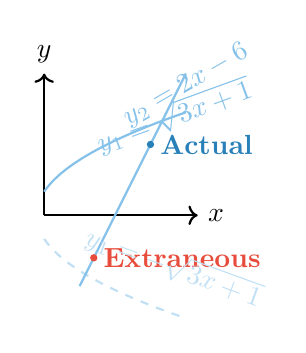
\begin{tikzpicture}[scale=0.3]
  % Axes
  \draw[->,thick] (0,0) -- (6.5,0) node[right] {$x$};
  \draw[->,thick] (0,0) -- (0,6) node[above] {$y$};
  % y1 = sqrt(3x+1) (top branch)
  \draw[thick,secondary!60,domain=0:6,samples=100] plot (\x,{sqrt(3*\x+1)});
  % y1 = -sqrt(3x+1) (bottom branch, dashed)
  \draw[thick,secondary!30,dashed,domain=0:6,samples=100] plot (\x,{-sqrt(3*\x+1)});
  % y2 = 2x-6
  \draw[thick,secondary!60,domain=1.5:6,samples=2] plot (\x,{2*\x-6});
  % Actual root (approximate)
  \filldraw[primary] (4.5,3) circle (0.13);
  \node[primary,right,font=\bfseries] at (4.5,3) {Actual};
  % Extraneous root (approximate)
  \filldraw[accent] (2.1,-1.8) circle (0.13);
  \node[accent,right,font=\bfseries] at (2.1,-1.8) {Extraneous};
  % Labels
  \node[secondary!60,rotate=20] at (5.5,4.2) {$y_1=\sqrt{3x+1}$};
  \node[secondary!30,rotate=-20] at (5.5,-2.2) {$y_1=-\sqrt{3x+1}$};
  \node[secondary!60,rotate=30] at (6,5.5) {$y_2=2x-6$};
\end{tikzpicture}
\end{columns}
\end{tcolorbox}
\end{frame}

\end{document} 